\documentclass[crop, tikz]{standalone}

\usepackage{tkz-base}
\usetikzlibrary {arrows.meta}

\begin{document}
    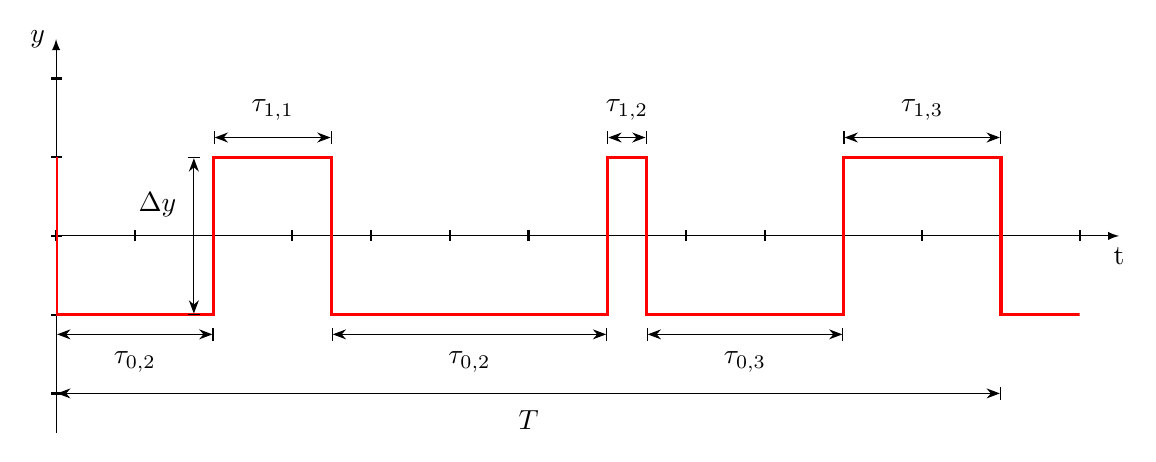
\begin{tikzpicture}[>=Stealth, scale=1]
        \tkzInit[xmax=13,ymax=2,xmin=0, ymin=-2.5]
        %\tkzGrid
        \tkzDrawY \tkzDrawX[label=t]% \tkzLabelX \tkzLabelY
        \tkzClip
        \draw [very thick,red]
            (0,1) -- ++ (0,-2) -- ++(2,0) -- ++(0,2) -- ++(1.5,0) -- ++(0,-2) -- ++(3.5,0) -- ++(0,2) -- ++(0.5,0) -- ++(0,-2) -- ++(2.5,0) -- ++(0,2) -- ++(2,0) -- ++(0,-2) -- ++(1,0)
        ;
        \draw [|<->|] (0,-1.25) -- node[below=1mm] {$\tau_{0,2}$} ++(2,0);
        \draw [|<->|] (2,1.25) -- node[above=1mm] {$\tau_{1,1}$} ++(1.5,0);
        \draw [|<->|] (3.5,-1.25) -- node[below=1mm] {$\tau_{0,2}$} ++(3.5,0);
        \draw [|<->|] (7,1.25) -- node[above=1mm] {$\tau_{1,2}$} ++(0.5,0);
        \draw [|<->|] (7.5,-1.25) -- node[below=1mm] {$\tau_{0,3}$} ++(2.5,0);
        \draw [|<->|] (10,1.25) -- node[above=1mm] {$\tau_{1,3}$} ++(2,0);
        \draw [|<->|] (1.75,-1) -- node[left=1mm, yshift=4mm] {$\Delta y$} ++(0,2);
        \draw [|<->|] (0,-2) -- node[below=1mm] {$T$} ++(12,0);
    \end{tikzpicture}
\end{document}
